\documentclass[12pt,a4paper]{article}
\usepackage[latin1]{inputenc}
\usepackage{amsmath}
\usepackage{amsfonts}
\usepackage{amssymb}
\usepackage{graphicx}
\usepackage{multirow,multicol}
\usepackage{pifont,hyperref,lastpage,fancyhdr,movie15,float}

\usepackage[utf8]{inputenc}   % Encodage UTF-8 (permet d’écrire les accents directement)
\usepackage[T1]{fontenc}      % Police adaptée aux caractères accentués
\usepackage[french]{babel}    % Adaptation typographique française (espaces, titres, etc.)

\usepackage{graphicx}   % Pour inclure des images avec \includegraphics
\usepackage{float}      % Pour mieux contrôler la position des images (option [H])

\usepackage[linesnumbered,ruled,vlined]{algorithm2e}
\usepackage[utf8]{inputenc}   % Encodage UTF-8
\usepackage[english]{babel}   % Langue anglaise

% Mathématiques et symboles
\usepackage{amsmath}          % Formules mathématiques avancées
\usepackage{amssymb}          % Symboles mathématiques
\usepackage{amsthm}           % Théorèmes, définitions, etc.

% Graphiques et images
\usepackage{graphicx}         % Inclure des images
\usepackage{float}            % Pour forcer le placement [H]

% Tableaux
\usepackage{booktabs}         % Tableaux avec \toprule, \midrule, \bottomrule

% Listes avancées
\usepackage{enumitem}         % Contrôle sur les listes

% TikZ pour les diagrammes et automates
\usepackage{tikz}
\usetikzlibrary{automata, positioning, arrows}

% Couleurs
\usepackage{xcolor}           % Pour colorier texte ou formes

% Hyperliens (optionnel)
\usepackage{hyperref}

\usepackage[left=3cm,right=3cm,top=4cm,bottom=3cm]{geometry}

%%%%%%%%%%%%%%%%%%%%%%%%%%%%%%%%%%%%%%%%%%%%%%%%%%%%%%%%%%%%%%%%%%%%%%%%%
%%%%%%%%%%%%%%%%%%%%%%%%%% Footer and Header %%%%%%%%%%%%%%%%%%%%%%%%%%%%
\pagestyle{fancy}                                                     %%%
\fancyhf{} 		                                                      %%%
\lfoot{\tiny\textsf{
\includegraphics[width=1.8cm]{AIMSSenegalLogo}    %%%
Po.Box~1418 Mbour-Thies,~phone~{(+221) 33 956 7693},~                 %%%
\url{http://www.aims-senegal.org}}}                                   %%%
\rfoot{\bfseries Page \thepage~of \pageref{LastPage}}                 %%%
\renewcommand{\footrulewidth}{1.pt}\renewcommand{\headrulewidth}{0pt} %%%
%%%%%%%%%%%%%%%%%%%%%%%%%%%%%%%%%%%%%%%%%%%%%%%%%%%%%%%%%%%%%%%%%%%%%%%%%
%%%%%%%%%%%%%%%%%%%%%%%%%%%%%%%%%%%%%%%%%%%%%%%%%%%%%%%%%%%%%%%%%%%%%%%%%

%%%%%%%%%%%%%%%%%%%%%%%%%%%%%%%%%%%%%%%%%%%%%%%%%%%%%%%%%%%%%%%%%%%%%%%%%
%%%%%%% Fill here information about the present assignment %%%%%%%%%%%%%%
\newcommand{\code}{Group 10}                                       %%%
\newcommand{\deadline}{[Date, Time]}                                  %%%
\newcommand{\assignment}{assignment 2 ON Programing with python}			  %%% 
\newcommand{\lecturer}{Lecturer: Dr Yae U Gaba, Quantum Leap Africa, AIMS RIC}                     %%%
%%%%%%%%%%%%%%%%%%%%%%%%%%%%%%%%%%%%%%%%%%%%%%%%%%%%%%%%%%%%%%%%%%%%%%%%%
%%%%%%%%%%%%%%%%%%%%%%%%%%%%%%%%%%%%%%%%%%%%%%%%%%%%%%%%%%%%%%%%%%%%%%%%%

%%%%%%%%%%%%%%%%%%%%%%%%%%%%%%%%%%%%%%%%%%%%%%%%%%%%%%%%%%%%%%%%%%%%%%%%%
%%%%%%%%%%%%%%%%%%%%%%  Title at the first page  %%%%%%%%%%%%%%%%%%%%%%%%
\title{\vspace*{-4cm}\begin{minipage}{\textwidth}                     %%%
\begin{center}                                                        %%%
\begin{tabular}{|c|c|c|}                                              %%%
\hline\multicolumn{3}{|c|}{\bf\scriptsize\MakeUppercase\assignment}\\ %%%
\hline{\small Student's Code}&                                        %%%
\multirow{3}{7cm}{
\includegraphics[width=7.5cm,height=2.3cm]{AIMSSenegalLogo}} %%%
& {\small Deadline}\\                                                 %%%
\cline{1-1}\cline{3-3}{\small\bf\code}&&{\small\bf\deadline} \\       %%%
\cline{1-1}\cline{3-3}{\small\today} &&{\small2025-2026}\\            %%%
\hline\multicolumn{3}{|r|}{\scriptsize\lecturer}\\\hline              %%%
\end{tabular}                                                         %%%
\end{center}                                                          %%%
\end{minipage}\hfill\date{}\vspace*{-1cm}}                            %%%
%%%%%%%%%%%%%%%%%%%%%%%%%%%%%%%%%%%%%%%%%%%%%%%%%%%%%%%%%%%%%%%%%%%%%%%%%
%%%%%%%%%%%%%%%%%%%%%%%%%%%%%%%%%%%%%%%%%%%%%%%%%%%%%%%%%%%%%%%%%%%%%%%%%

\newcommand{\K}{\mathbb{K}}
\newcommand{\R}{\mathbb{R}}
\newcommand{\C}{\mathbb{C}}

\newtheorem{theo}{Theorem}
\newtheorem{defi}{Definition}
\newenvironment{proof}[1][Proof.]{\textbf{#1~}}{\ \rule{0.5em}{0.5em}}

\begin{document}
\maketitle\thispagestyle{fancy}

\setlength{\tabcolsep}{8pt} % Adds horizontal padding (default is 6pt)
\renewcommand{\arraystretch}{1} % Adds vertical padding between rows

\begin{table}[H]
\centering
\caption{List of Group Members}
\begin{tabular*}{\textwidth}{@{\extracolsep{\fill}}|c|l|}
\hline
\
\textbf{No.} & \textbf{Full Name} \\ \hline
1 & CHEMEGNIE SOFFO Clarisse \\ \hline
2 & Malick Ka \\ \hline
3 & GNINTEZEMO MAMEKEM ROSLY \\ \hline
4 & Aballo Geraldo Roy \\ \hline
5 & Soukeye Toure \\ \hline
\end{tabular*}
\end{table}


\section{Introduction}

The detection of vehicle license plates is a classic problem in pattern recognition and text analysis. 
In the context of Senegal, license plates follow specific standardized formats, such as 
\texttt{XY-1234-T} or \texttt{XY-1234-ZT}, where \texttt{X, Y, Z, T} represent uppercase letters 
and \text{1 to 4} represent digits. Identifying these patterns accurately within arbitrary text strings 
is important for various applications, such as data extraction, document analysis, and automated 
information verification.

This project, titled \textit{License Plate Detection}, aims to design and implement a Python-based 
system capable of detecting Senegalese vehicle license plate numbers within any textual input. 
The system should output a Boolean indicating the presence of one or more plates, and if found, 
it should display the detected license plates in their canonical normalized form.

To address this challenge, two distinct approaches were implemented and compared:
\begin{itemize}
    \item \textbf{Parsing-based detection:} a direct approach that scans and parses the text to identify 
    character patterns consistent with the license plate format.
    \item \textbf{Deterministic Finite Automaton (DFA)-based detection:} a formal approach relying on 
    automata theory to model valid transitions and recognize plates based on state transitions.
\end{itemize}

The main objective is to evaluate and compare both methods in terms of their implementation 
complexity, execution time, and scalability. The system should also handle practical constraints, 
such as case insensitivity, tolerance to punctuation, and the ability to normalize detected plates 
to uppercase with standardized hyphenation.

Through this work, we explore how traditional string parsing techniques and theoretical formal 
language models can be applied to real-world text processing problems, highlighting their respective 
advantages, limitations, and potential for integration in larger natural language or data analysis systems.

\newpage

\section{Specifications and Constraints}

\subsection{Description of the Senegalese License Plate Format}
Senegalese vehicle license plates follow a standardized structure that combines letters and digits.
The official formats considered in this project are:
\[
\texttt{XY-1234-T} \quad \text{or} \quad \texttt{XY-1234-ZT}
\]
where:
\begin{itemize}
    \item \texttt{X, Y, Z, T} are uppercase alphabetic characters (\texttt{A--Z}),
    \item \texttt{1, 2, 3, 4} are numerical digits (\texttt{0--9}),
    \item and each block is separated by either a hyphen (\texttt{-}) or a space (\texttt{ }).
\end{itemize}

\subsection{Program Inputs and Outputs}
\begin{itemize}
    \item \textbf{Input:} an arbitrary text string possibly containing one or more license plates.
    \item \textbf{Output:}
    \begin{enumerate}
        \item a Boolean indicating whether valid plates were found,
        \item the list of detected plates (without duplicates),
        \item and the total number of unique plates detected.
    \end{enumerate}
\end{itemize}

\subsection{Functional Rules and Requirements}
\begin{itemize}
    \item \textbf{Case insensitivity:} detection must work regardless of case.
    \item \textbf{Flexible separators:} plates may use hyphens or spaces.
    \item \textbf{Invalid substring exclusion:} no detection inside longer words.
    \item \textbf{Punctuation tolerance:} commas, periods, or other punctuation marks around plates must be ignored.
    \item \textbf{Clear display:} plates must be displayed in uppercase and normalized form (e.g., \texttt{XY-1234-T}).
    \item \textbf{Interactive menu:} the program should allow multiple tests until the user chooses to exit.
\end{itemize}

\subsection{Technical Constraints}
\begin{itemize}
    \item The project must be implemented in \textbf{pure Python}, without any external libraries or imports.
    \item The code should remain clear, well-commented, and executable on any standard Python interpreter.
    \item Algorithmic complexity should remain reasonable.

\end{itemize}

\section{Methodology and Implementation}

In this section, we will discuss two different methods used to detect Senegalese vehicle license plates: 
the \textit{string parsing} approach and the \textit{automaton-based} approach. 


\subsection{Method One  String Parsing}


Parsing, in general, is the process of analyzing a sequence of symbols in order to understand its structure 
and extract meaningful information. It is commonly used in text processing, compilers, and data extraction. 
The main idea is to read the input text sequentially, character by character, and identify patterns or tokens 
according to predefined rules.

In the context of license plate detection, string parsing consists of scanning the text to recognize sequences 
that match the expected format of Senegalese plates (e.g., \texttt{XY-1234-T} or \texttt{XY-1234-ZT}). 




\begin{figure}[H]
    \centering
    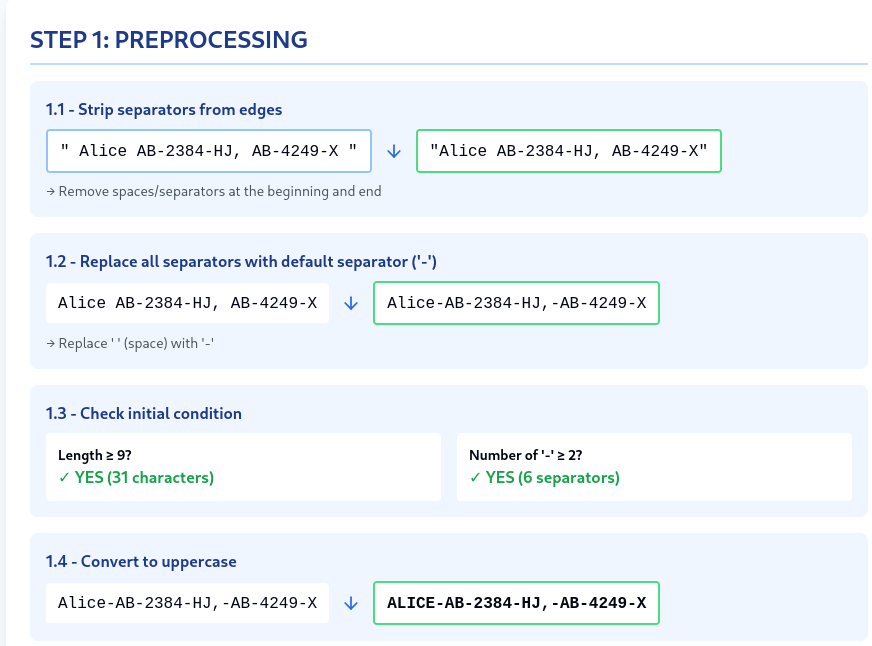
\includegraphics[width=\linewidth]{AIMS_Senegal__Assignment_template/step1Parsing.png}
    \caption{Input preprocessing and normalization.}
    \label{fig:step1Parsing}

\end{figure}

\textbf{Step 1: Pattern Scanning} \\
The input string is cleaned and normalized. Extra spaces and separators are removed, all separators are unified to ``-``, and the text is converted to uppercase. This ensures a consistent format for pattern detection.




\begin{figure}[H]
    \centering
    \includegraphics[width=\linewidth]{AIMS_Senegal__Assignment_template/step2Parsing.png}
    \caption{Pattern Search}
    \label{fig:step1Parsing}
\end{figure}

\begin{figure}[H]
    \centering
    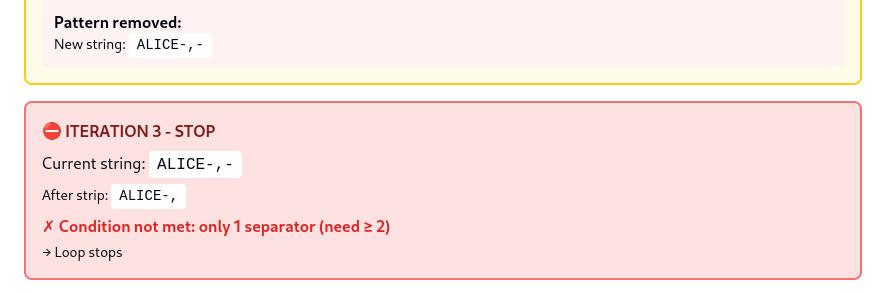
\includegraphics[width=\linewidth]{step2-1parsing.png}
    \caption{Pattern Search Iterration}
    \label{fig:step1Parsing}
\end{figure}


\textbf{Step 2: Pattern Scanning} \\
The algorithm scans the string character by character, looking for patterns that match the structure \texttt{XX-####-X(X)}. Each valid pattern is extracted and removed from the string iteratively until no more patterns can be found.


\begin{figure}[H]
    \centering
    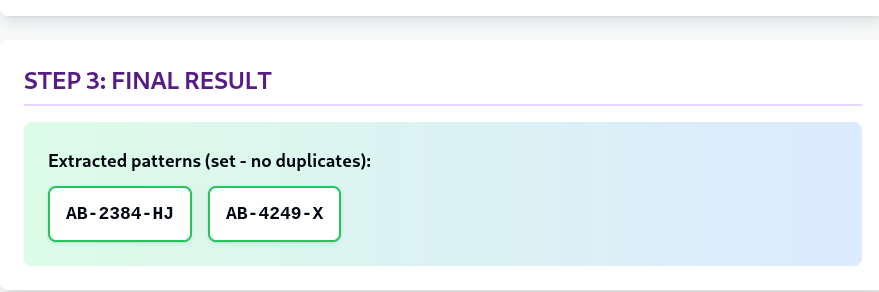
\includegraphics[width=\linewidth]{step3parsing.png}
    \caption{Final result}
    \label{fig:step1Parsing}
\end{figure}
\text{All extracted patterns are collected into a set to avoid duplicates. The final output displays all unique patterns found in the original input.}\\

\textbf{Workflow/ Summary And Algorithm} \\
The process combines preprocessing, iterative pattern search, extraction, and condition checking to reliably detect structured sequences within a string, returning only valid, unique patterns.

\begin{figure}[h]
    \centering
    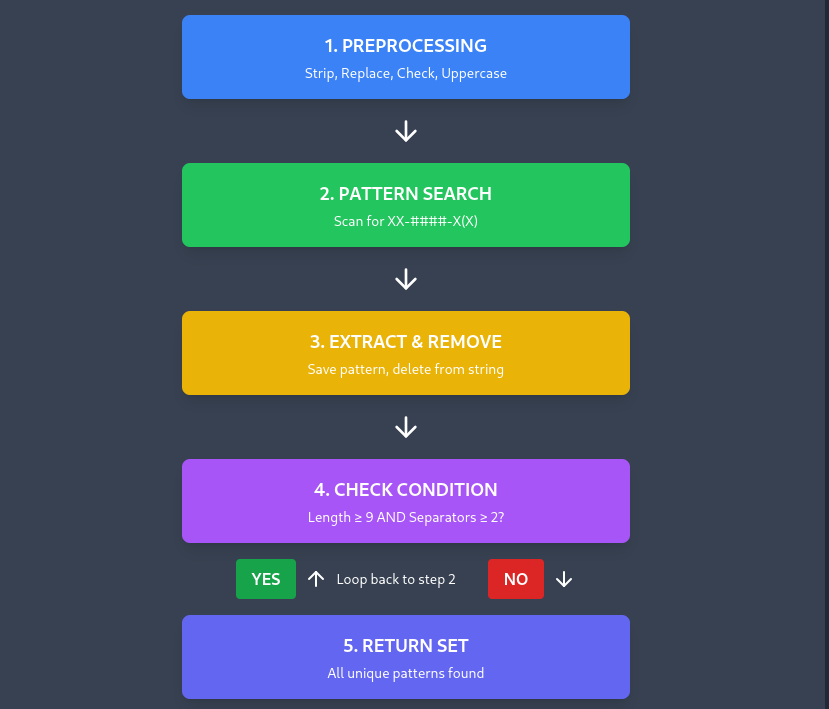
\includegraphics[width=\linewidth]{AIMS_Senegal__Assignment_template/summaryParsing.png}
    \caption{Workflow}
    \label{fig:step1Parsing}
\end{figure}


\begin{algorithm}[H]
\caption{Parsing-Based License Plate Detection}
\KwIn{Input string $text$}
\KwOut{Set of all detected license plates $patterns$}

$patterns \gets \emptyset$\;
Clean and normalize separators in $text$ (replace spaces with '-')\;
Convert all letters in $text$ to uppercase\;

\While{$length(text) \geq 9$ \textbf{and} number of '-' in $text \geq 2$}{
    \For{each character $c$ in $text$}{
        \If{$c$ is '-' \textbf{and} pattern $XX-####-X(X)$ exists around $c$}{
            Extract the pattern\;
            Add it to $patterns$\;
            Remove the extracted pattern from $text$\;
            \textbf{break} inner loop\;
        }
    }
    Strip leading and trailing separators from $text$\;
}

\Return $patterns$\;
\end{algorithm}


\subsection{Method Two Deterministic Finite Automaton (DFA)}



\subsection{Definition of an Automaton}

An \textbf{automaton} is a theoretical model used in computer science to describe a system that processes 
a sequence of inputs and changes its internal state accordingly. It consists of a set of states, an 
alphabet of symbols it can read, transition rules that define how the automaton moves from one state 
to another based on input symbols, and one or more designated final (or accepting) states. 

\subsection{Definition of Alphabets}

\subsubsection{Formal Sets}

We define the following sets:

\begin{align}
    \alpha &= \{A, B, C, \ldots, Z, a, b, c, \ldots, z\} \quad \text{(letters)} \\
    \beta &= \{0, 1, 2, 3, 4, 5, 6, 7, 8, 9\} \quad \text{(digits)} \\
    \theta &= \{\text{-}, \text{ }\} \quad \text{(separators: hyphen or space)} \\
    \varepsilon &= \text{empty string} \\
    \Delta &= \{\text{.}, \text{,}, \text{!}, \text{?}, \text{;}, \text{:}, \ldots\} \quad \text{(punctuation)}
\end{align}



\subsubsection{Deterministic Finite Automaton (DFA)}

\subsubsection{Formal Definition}

The automaton is defined by the quintuple:
\[
\mathcal{A} = (Q, \Sigma, \delta, q_0, F)
\]

where:
\begin{itemize}
    \item $Q = \{Q_0, Q_1, Q_2, Q_3, Q_4, Q_5, Q_6, Q_7\}$ is the set of states
    \item $\Sigma$ is the alphabet defined above
    \item $\delta : Q \times \Sigma \rightarrow Q$ is the transition function
    \item $q_0 = Q_0$ is the initial state
    \item $F = \{Q_7\}$ is the set of final (accepting) states
\end{itemize}

\subsubsection{Description of States}

\begin{itemize}[leftmargin=2cm]
    \item[$Q_0$:] Initial state. Ignores initial delimiters ($\varepsilon$, $\Delta$, $\theta$).
    \item[$Q_1$:] Two initial letters read (XY).
    \item[$Q_2$:] First separator validated, waiting for digits.
    \item[$Q_3$:] Four digits read (abcd).
    \item[$Q_4$:] Second separator validated, waiting for final letter(s).
    \item[$Q_5$:] One final letter read, format \texttt{XY-abcd-T}.
    \item[$Q_6$:] Two final letters read, format \texttt{XY-abcd-ZT}.
    \item[$Q_7$:] Accepting state. Valid license plate detected.
\end{itemize}

\subsubsection{Transition Function}

\subsubsection{Transition Table $\delta$}

\begin{table}[H]
\centering
\begin{tabular}{@{}cccl@{}}
\toprule
\textbf{State} & \textbf{Symbol} & \textbf{Next State} & \textbf{Description} \\
\midrule
$Q_0$ & $\alpha^2$ & $Q_1$ & Read 2 letters (XY) \\
$Q_0$ & $\varepsilon \cup \Delta \cup \theta$ & $Q_0$ & Ignore initial delimiters \\
$Q_1$ & $\theta$ & $Q_2$ & Separator after letters \\
$Q_2$ & $\beta^4$ & $Q_3$ & Read 4 digits (abcd) \\
$Q_3$ & $\theta$ & $Q_4$ & Separator after digits \\
$Q_4$ & $\alpha^1$ & $Q_5$ & 1 final letter (T) \\
$Q_4$ & $\alpha^2$ & $Q_6$ & 2 final letters (ZT) \\
$Q_5$ & $\varepsilon \cup \Delta \cup \theta$ & $Q_7$ & End of format XY-abcd-T \\
$Q_6$ & $\varepsilon \cup \Delta \cup \theta$ & $Q_7$ & End of format XY-abcd-ZT \\
\bottomrule
\end{tabular}
\caption{Transition function $\delta$ of the automaton}
\label{tab:transition}
\end{table}

\subsubsection{Graphical Representation of the Automaton}

\begin{figure}[H]
\centering
\begin{tikzpicture}[->,>=Stealth,shorten >=1pt,auto,node distance=3cm,
                    thick,main node/.style={circle,draw,font=\sffamily\Large\bfseries}]

  \node[state,initial] (q0) {$Q_0$};
  \node[state] (q1) [right of=q0] {$Q_1$};
  \node[state] (q2) [right of=q1] {$Q_2$};
  \node[state] (q3) [below of=q2] {$Q_3$};
  \node[state] (q4) [left of=q3] {$Q_4$};
  \node[state] (q5) [below left of=q4] {$Q_5$};
  \node[state] (q6) [below right of=q4] {$Q_6$};
  \node[state,accepting] (q7) [below of=q4] {$Q_7$};

  \path[every node/.style={font=\sffamily\small}]
    (q0) edge [loop above] node {$\varepsilon, \Delta, \theta$} (q0)
         edge node {$\alpha^2$} (q1)
    (q1) edge node {$\theta$} (q2)
    (q2) edge node {$\beta^4$} (q3)
    (q3) edge node {$\theta$} (q4)
    (q4) edge node {$\alpha^1$} (q5)
         edge node [above right] {$\alpha^2$} (q6)
    (q5) edge node [up] {$\varepsilon, \Delta, \theta$} (q7)
    (q6) edge node [dnow] {$\varepsilon, \Delta, \theta$} (q7);
\end{tikzpicture}
\caption{Diagram of the deterministic finite automaton}
\label{fig:automaton}
\end{figure}

\begin{algorithm}[H]
\caption{DFA-based Senegalese License Plate Detection}
\label{alg:dfa_plates}
\KwData{Input text string $text$}
\KwResult{Set of normalized plates detected in the text}

\SetKwFunction{FMain}{DFA\_Plate\_Detection}
\SetKwProg{Fn}{Function}{:}{}
\Fn{\FMain{$text$}}{
    \tcp{Define character sets}
    $\alpha \gets$ letters A-Z, a-z\;
    $\beta \gets$ digits 0-9\;
    $\theta \gets \{-, \text{space}\}$\;
    $\epsilon \gets \{\text{empty string}\}$\;
    $\delta \gets$ punctuation and special characters\;
    $\sigma \gets \alpha \cup \beta \cup \theta \cup \epsilon \cup \delta$\;
    
    \tcp{Initialize empty set for plates}
    $plates \gets \{\}$\;
    
    \tcp{Sliding window scan}
    \For{$i \gets 0$ \KwTo $|text|-1$}{
        $word1 \gets text[i:i+9]$\;
        $word2 \gets text[i:i+10]$\;
        
        \If{accept(word1)}{
            $plates \gets plates \cup \{word1\}$\;
        }
        \If{accept(word2)}{
            $plates \gets plates \cup \{word2\}$\;
        }
    }
    $normalized\_plates \gets$ Clean\_And\_Normalize($plates$)

    \Return $normalized\_plates$\;
}
\end{algorithm}




\newpage

\section{Comparative Study of the Two Approaches}

The project implements two distinct methods for detecting Senegalese license plates in text: \textbf{manual parsing} and \textbf{deterministic finite automaton (DFA)}. Both approaches aim to recognize patterns of the form \texttt{XY-1234-T} or \texttt{XY-1234-ZT}, but they differ in methodology, complexity, and performance characteristics.

\subsection{Manual Parsing}

\begin{itemize}
    \item \textbf{Principle:} This method analyzes the input string character by character, looking for separators (\texttt{-} or space) and validating the pattern in a procedural manner.
    \item \textbf{Strengths:} 
        \begin{itemize}
            \item Straightforward implementation in Python.
            \item Easy to understand and modify for small-scale applications.
            \item Directly handles normalization and extraction of detected plates.
        \end{itemize}
    \item \textbf{Limitations:} 
        \begin{itemize}
            \item Algorithmic complexity grows with string length.
            \item Manual checks make it prone to human error for more complex or variable formats.
            \item Less structured and harder to extend to new patterns.
        \end{itemize}
\end{itemize}

\subsection{Deterministic Finite Automaton (DFA)}

\begin{itemize}
    \item \textbf{Principle:} The DFA approach models the detection process as a set of states, transitions, and acceptance conditions. Each character is processed according to the current state and the type of character (letter, digit, separator, or punctuation).
    \item \textbf{Strengths:} 
        \begin{itemize}
            \item Provides a formal and systematic way to recognize patterns.
            \item Easier to reason about correctness, especially for complex patterns.
            \item Can be extended to multiple formats by adding states or transitions.
        \end{itemize}
    \item \textbf{Limitations:} 
        \begin{itemize}
            \item More elaborate to implement initially.
            \item Debugging may require careful tracing of states.
            \item Slightly higher memory usage due to state management.
        \end{itemize}
\end{itemize}

\subsection{Comparison Summary}

\begin{table}[H]
\centering
\begin{tabular}{lcc}
\toprule
\textbf{Criterion} & \textbf{Parsing} & \textbf{DFA} \\
\midrule
Implementation simplicity & High & Moderate \\
Formal structure & Low & High \\
Ease of extension & Low & High \\
Time Complexity & $O(n)$ & $O(n)$ \\ 
Performance on long texts & Moderate & High \\
Error resilience & Moderate & High \\
Readability & High for small code & Moderate \\
\bottomrule
\end{tabular}
\caption{Comparison of manual parsing and DFA approaches}
\label{tab:comparison}
\end{table}

\textbf{Conclusion:} Both methods correctly detect Senegalese license plates. For short scripts or simple tasks, manual parsing is sufficient. For robust, scalable, and formally verifiable solutions, the DFA approach is recommended, as it enforces structure, reduces errors, and allows easier extension to other formats.

\newpage
\section{Application}

\begin{figure}
    \centering
    \includegraphics[width=1\linewidth]{}
    \caption{Enter Caption}
    \label{fig:placeholder}
\end{figure}

\begin{figure}[H]
    \centering
    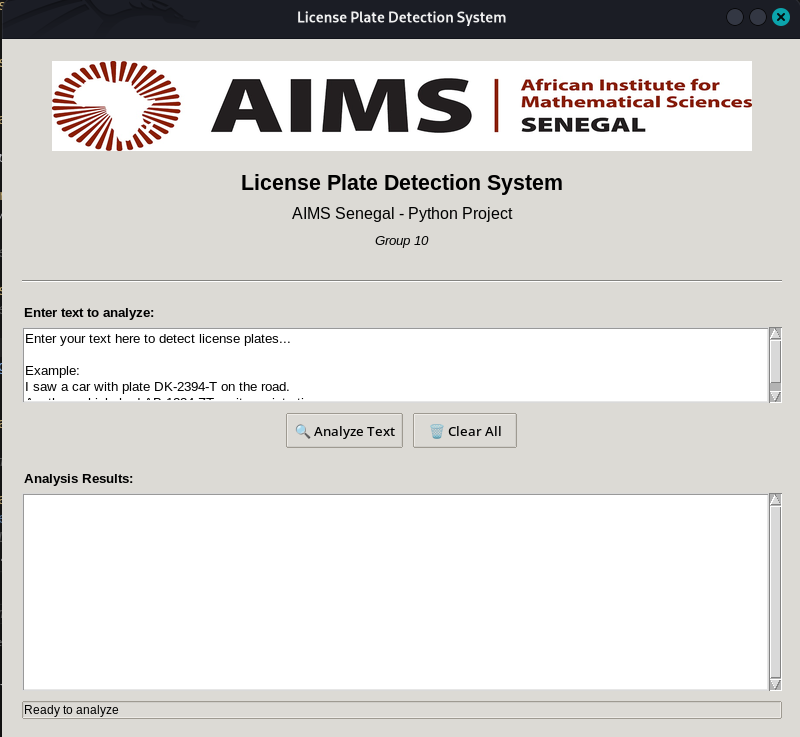
\includegraphics[width=\linewidth]{AIMS_Senegal__Assignment_template/app.png}
    \caption{APLLICATION.}
    \label{fig:step1Parsing}
\end{figure}

\text{Code oepen source at https://github.com/ioget/AIMS-PP-Group-10}

\end{document}


